\let\negmedspace\undefined
\let\negthickspace\undefined

\documentclass[journal,12pt,onecolumn]{IEEEtran}
%\documentclass[journal,12pt,twocolumn]{IEEEtran}
%
\usepackage{setspace}
\usepackage{gensymb}
%\doublespacing
\singlespacing

%\usepackage{graphicx}
%\usepackage{amssymb}
%\usepackage{relsize}
\usepackage[cmex10]{amsmath}
%\usepackage{amsthm}
%\interdisplaylinepenalty=2500
%\savesymbol{iint}
%\usepackage{txfonts}
%\restoresymbol{TXF}{iint}
%\usepackage{wasysym}
\usepackage{amsthm}
\usepackage{mathrsfs}
\usepackage{txfonts}
\usepackage{stfloats}
\usepackage{cite}
\usepackage{cases}
\usepackage{subfig}
%\usepackage{xtab}
\usepackage{longtable}
\usepackage{multirow}
%\usepackage{algorithm}
%\usepackage{algpseudocode}
\usepackage{enumitem}
\usepackage{mathtools}
\usepackage{tikz}
\usepackage{circuitikz}
\usepackage{verbatim}
\usepackage{hyperref}
%\usepackage{stmaryrd}
\usepackage{tkz-euclide} % loads  TikZ and tkz-base
%\usetkzobj{all}
\usepackage{listings}
\usepackage{color}                                            %%
\usepackage{array}                                            %%
\usepackage{longtable}                                        %%
\usepackage{calc}                                             %%
\usepackage{multirow}                                         %%
\usepackage{hhline}                                           %%
\usepackage{ifthen}                                           %%
%optionally (for landscape tables embedded in another document): %%
\usepackage{lscape}     
\usepackage{multicol}
\usepackage{chngcntr}
\usepackage{iftex}
%\usepackage[latin9]{inputenc}
\usepackage{geometry}
\usepackage{bm}
%\geometry{verbose,tmargin=2cm,bmargin=3cm,lmargin=1.8cm,rmargin=1.5cm,headheight=2cm,headsep=2cm,footskip=3cm}
\usepackage{array}
\newcolumntype{L}[1]{>{\raggedright\let\newline\\\arraybackslash\hspace{0pt}}m{#1}}
\newcolumntype{C}[1]{>{\centering\let\newline\\\arraybackslash\hspace{0pt}}m{#1}}
\newcolumntype{R}[1]{>{\raggedleft\let\newline\\\arraybackslash\hspace{0pt}}m{#1}}

%\usepackage{graphicx}
%\usepackage{setspace}
%\usepackage{parskip}

\def \hsp {\hspace{3mm}}

\makeatletter

\providecommand{\tabularnewline}{\\}



\makeatother
\ifxetex
\usepackage[T1]{fontenc}
\usepackage{fontspec}
%\setmainfont[ Path = fonts/]{Sanskrit_2003.ttf}
\newfontfamily\nakulafont[Script=Devanagari,AutoFakeBold=2,Path = fonts/]{Nakula}
%\newfontfamily\liberationfont{Liberation Sans Narrow}
%\newfontfamily\liberationsansfont{Liberation Sans}
\fi
\usepackage{tikz}
\usepackage{xcolor}
%\usepackage{enumerate}

%\usepackage{wasysym}
%\newcounter{MYtempeqncnt}
\DeclareMathOperator*{\Res}{Res}
%\renewcommand{\baselinestretch}{2}
\renewcommand\thesection{\arabic{section}}
\renewcommand\thesubsection{\thesection.\arabic{subsection}}
\renewcommand\thesubsubsection{\thesubsection.\arabic{subsubsection}}

\renewcommand\thesectiondis{\arabic{section}}
\renewcommand\thesubsectiondis{\thesectiondis.\arabic{subsection}}
\renewcommand\thesubsubsectiondis{\thesubsectiondis.\arabic{subsubsection}}

% correct bad hyphenation here
\hyphenation{op-tical net-works semi-conduc-tor}
\def\inputGnumericTable{}                                 %%

\lstset{
	language=tex,
	frame=single, 
	breaklines=true
}

%\begin{document}
%


\newtheorem{theorem}{Theorem}[section]
\newtheorem{problem}{Problem}
\newtheorem{proposition}{Proposition}[section]
\newtheorem{lemma}{Lemma}[section]
\newtheorem{corollary}[theorem]{Corollary}
\newtheorem{example}{Example}[section]
\newtheorem{definition}[problem]{Definition}
%\newtheorem{thm}{Theorem}[section] 
%\newtheorem{defn}[thm]{Definition}
%\newtheorem{algorithm}{Algorithm}[section]
%\newtheorem{cor}{Corollary}
\newcommand{\BEQA}{\begin{eqnarray}}
	\newcommand{\EEQA}{\end{eqnarray}}
\newcommand{\define}{\stackrel{\triangle}{=}}
\bibliographystyle{IEEEtran}
%\bibliographystyle{ieeetr}
\providecommand{\mbf}{\mathbf}
\providecommand{\pr}[1]{\ensuremath{\Pr\left(#1\right)}}
\providecommand{\qfunc}[1]{\ensuremath{Q\left(#1\right)}}
\providecommand{\sbrak}[1]{\ensuremath{{}\left[#1\right]}}
\providecommand{\lsbrak}[1]{\ensuremath{{}\left[#1\right.}}
\providecommand{\rsbrak}[1]{\ensuremath{{}\left.#1\right]}}
\providecommand{\brak}[1]{\ensuremath{\left(#1\right)}}
\providecommand{\lbrak}[1]{\ensuremath{\left(#1\right.}}
\providecommand{\rbrak}[1]{\ensuremath{\left.#1\right)}}
\providecommand{\cbrak}[1]{\ensuremath{\left\{#1\right\}}}
\providecommand{\lcbrak}[1]{\ensuremath{\left\{#1\right.}}
\providecommand{\rcbrak}[1]{\ensuremath{\left.#1\right\}}}
\theoremstyle{remark}
\newtheorem{rem}{Remark}
\newcommand{\sgn}{\mathop{\mathrm{sgn}}}
\providecommand{\abs}[1]{\left\vert#1\right\vert}
\providecommand{\res}[1]{\Res\displaylimits_{#1}} 
\providecommand{\norm}[1]{\left\lVert#1\right\rVert}
%\providecommand{\norm}[1]{\lVert#1\rVert}
\providecommand{\mtx}[1]{\mathbf{#1}}
\providecommand{\mean}[1]{E\left[ #1 \right]}
\providecommand{\fourier}{\overset{\mathcal{F}}{ \rightleftharpoons}}
%\providecommand{\hilbert}{\overset{\mathcal{H}}{ \rightleftharpoons}}
%\providecommand{\system}{\overset{\mathcal{H}}{ \longleftrightarrow}}
\providecommand{\system}[1]{\overset{\mathcal{#1}}{ \longleftrightarrow}}
\providecommand{\gauss}[2]{\mathcal{N}\ensuremath{\left(#1,#2\right)}}
%
%\newcommand{\solution}[2]{\textbf{Solution:}{#1}}
\newcommand{\solution}{\noindent \textbf{Solution: }}
\newcommand{\cosec}{\,\text{cosec}\,}
\newcommand{\sinc}{\,\text{sinc}\,}
\newcommand{\rect}{\,\text{rect}\,}
\providecommand{\dec}[2]{\ensuremath{\overset{#1}{\underset{#2}{\gtrless}}}}
\newcommand{\myvec}[1]{\ensuremath{\begin{pmatrix}#1\end{pmatrix}}}
\newcommand{\mydet}[1]{\ensuremath{\begin{vmatrix}#1\end{vmatrix}}}
\newcommand*{\permcomb}[4][0mu]{{{}^{#3}\mkern#1#2_{#4}}}
\newcommand*{\perm}[1][-3mu]{\permcomb[#1]{P}}
\newcommand*{\comb}[1][-1mu]{\permcomb[#1]{C}}
%\numberwithin{equation}{section}
\numberwithin{equation}{section}
%\numberwithin{problem}{section}
%\numberwithin{definition}{section}
\makeatletter
\@addtoreset{figure}{problem}
\makeatother
%\let\StandardTheFigure\thefigure
\let\vec\mathbf
%\renewcommand{\thefigure}{\theproblem.\arabic{figure}}
\renewcommand{\thefigure}{\arabic{section}.\arabic{figure}}
%\setlist[enumerate,1]{before=\renewcommand\theequation{\theenumi.\arabic{equation}}
	%\counterwithin{equation}{enumi}
	%\renewcommand{\theequation}{\arabic{subsection}.\arabic{equation}}
\let\StandardTheFigure\thefigure
	\vspace{3cm}
	%\usepackage{babel}
  \begin{document}
    \title{Random Forest}
    \maketitle
    \author{ Mannem Charan AI21BTECH11019}
    \begin{abstract}
     This report consists of my basic understanding of one of the popular Ml methods "Random Forest".
    \end{abstract}
    \section{Random Forest}
     Random Forest is a supervised machine learning algorithm used to solve classification and regression problems but more preffered for classification problems.It has quite an applications in bank sector,stock market and so on.It comes under non-parametric machine learning as the model will not assume any relationship between dependent and independent variables.As the name suggests, random forest simply generates decision trees on different training data subsets and takes their majority vote for predicting the outcome. This type of learning is known as "\textbf{Ensemble learning}".
    \section{Ensemble Learning}
      Ensemble learning is the process of combining multiple classifiers to solve a complex problem and to improve the performance of model.So in this case the final output predicted is based on the predictions of many individual classifiers. In general, ensemble learning uses two kinds of methods,
             \begin{enumerate}
               \item Bagging
               \item Boosting
             \end{enumerate}
    \textbf{Bagging:} In this method, the classifiers are trained with training samples which are subsets of training data which are randomly taken with replacement. So the same data points can be present in two or more classifiers.The output is based on majority voting.\\
    \textbf{Boosting :} In Boosting the weak learners are combined squentially to form a strong learner.By the word sequential we mean each model tries to compensate the weakness of the predecessor.\\
 In this case, random forest follows bagging method to do ensemble learning.
    \section{Understanding Random Forest}
      As we discussed earlier,Random forest generates the decision trees and predicts based on the outcomes of individual trees.So increasing the number of decision trees will decrease the possibilty of overfitting and increase the performance of model.The figure $\ref{Fig 1}$ shows how the outcome is predicted in random forest.
               \begin{figure}
                \centering
                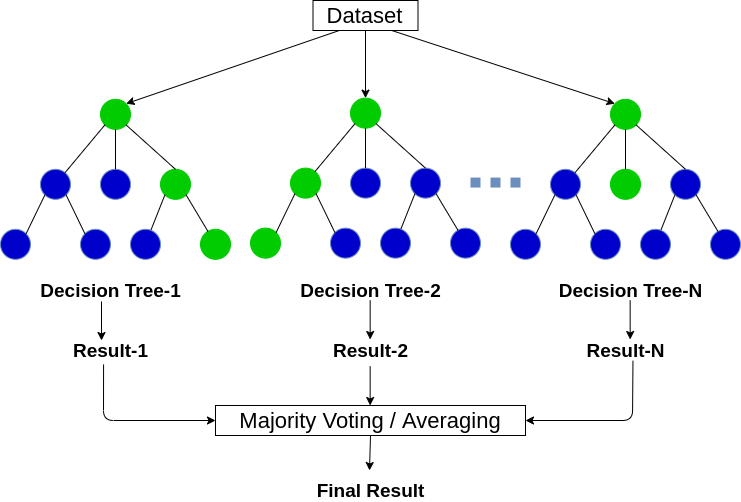
\includegraphics[width = 10cm]{randomforest.png}
                \caption{Predicting the outcome by random forest}
                \label{Fig 1}
               \end{figure}
 The process of dividing the training data randomly into different subsets with replacements is known as row sampling.The step that involves row sampling is known as "Bootstraping".After each model trained independently, they all predict the output for a commom data and majority of them is taken as final output. This step is known as "Aggregation".
    \section{Advantages of Random Forest}\label{advantages}
     \begin{enumerate}
       \item Decision trees are tend to have risk of overfitting as they are more dependent on training data.So,by combining the decision trees we are able to decrease the risk of overfitting as averaging the outcomes of individual trees decreases the prediction error.
       \item It runs efficiently on large data bases.
       \item Robust against the outliers since they are averaged out in the aggregation step.
     \end{enumerate}
    \section{Disadvantages of Random Forest}
     \begin{enumerate}
       \item It is hard to interpret the final outcome since we don't know exactly what features are responsible for the output as in decision trees.
       \item Sometimes it becomes hard to build a random forest due to limited computational power.
     \end{enumerate}
    \section{Miscellaneous}
      \begin{itemize}
        \item Random forest expect it's decision trees to have low correlation values among themselves.
        \item The features to be taken for decision trees should represent the target attribute since we are trying produce accurate results not to guess the result.
      \end{itemize}
    \section{Quesions}
      \begin{enumerate}
        \item What is ensemble learning?
        \item Which method does random forest follow while doing ensmeble learning?
        \item How random forest predicts the outcome of a data?
        \item What will happen if the decision trees have high correlation values?
        \item Give some advantages of random forest
      \end{enumerate}
    \section{Solutions}
       \begin{enumerate}
         \item The ensemble learning is the process of combining multiple classifiers which helps in improving the performance of model.
         \item The random forest follows bagging method in ensemble learning, it parallely trains the decision trees with data samples taken from data set with replacement.
         \item Random forest averages/takes the majority of outcomes predicted by the individual decision trees.
         \item If the decision trees with high correlation values predicting the outcome then there will be more variance and prediction error.As it will be no different from a single decision tree.
         \item Refer the section $\ref{advantages}$
       \end{enumerate}
    \end{document}
      
